\documentclass[final,5p,times,twocolumn]{elsarticle}

\usepackage{amsmath,amssymb,amsfonts}
\usepackage{graphicx}
\usepackage{booktabs}
\usepackage{multirow}
\usepackage{url}
\usepackage{hyperref}
\usepackage{color,xcolor}
\usepackage{tabularx}

\journal{Computers \& Security}

\begin{document}

\begin{frontmatter}

\title{DownstreamSec: Dissecting and Predicting Vulnerability Propagation and Security Exposure Across Upstream and Downstream Operating System Ecosystems}

\author[inst1]{Author Name\corref{cor1}}
\ead{author@institution.edu}
\cortext[cor1]{Corresponding author}

\author[inst1]{Co-Author Name}
\ead{coauthor@institution.edu}

\affiliation[inst1]{organization={Department of Computer Science and Engineering, University / Research Institute},
            city={City},
            postcode={PostalCode},
            country={Country}}

\begin{abstract}
When a critical vulnerability in the Linux kernel is resolved upstream, modern software supply chains operate under an implicit assumption: downstream operating system distributions promptly adopt the remediation and protect end-user systems. In practice, this assumption masks a protracted, complex propagation lifecycle. Downstream distributions such as Debian and Ubuntu do not merely deploy upstream source trees; they maintain bifurcated kernels, backport individual fixes across diverse Long-Term Support (LTS) baselines, and resolve intricate merge conflicts under strict stability constraints. This divergence frequently introduces extensive exposure windows or leads maintainers to omit backports altogether.

In this work, we present \textbf{DownstreamSec}, a comprehensive empirical study and predictive modeling framework analyzing vulnerability propagation from the Linux kernel to downstream enterprise distributions. We curate a multi-ecosystem dataset comprising all \textbf{9,208 common vulnerabilities} disclosed between 2005 and 2025 across upstream Linux, NVD, the Debian Security Tracker, and the Ubuntu Security Tracker, encompassing \textbf{55,248 evaluated downstream operating system release instances} with strictly zero synthetic data. We formalize a seven-state taxonomy ($D0$--$D6$) capturing nuanced downstream security postures, including clean upstream merges and modified backports. 

Our empirical measurement reveals that downstream remediation is fraught with systemic delays: across 40,198 resolved vulnerabilities, the median patch latency is \textbf{258.8 days} (mean 306.6 days), with \textbf{69.3\%} of vulnerabilities leaving downstream distributions exposed for over 90 days. Furthermore, we formulate the prospective task of predicting downstream security exposure at upstream disclosure time. Using strictly pre-remediation signals under an anti-leakage temporal split ($\le$2023 train vs. $\ge$2024 test), our models forecast downstream exposure with an \textbf{ROC-AUC of 0.8072} and \textbf{76.74\% balanced accuracy}. Feature attribution demonstrates that upstream stable tree backport volume and downstream kernel baseline distance dominate propagation outcomes. Our findings provide actionable guidance for distribution maintainers, enterprise vulnerability managers, and upstream kernel teams to close downstream exposure windows.
\end{abstract}

\begin{graphicalabstract}
\centering

\includegraphics[width=\columnwidth]{figures/fig1_survival_remediation_latency.pdf}
\end{graphicalabstract}

\begin{highlights}
\item Constructed a longitudinal multi-ecosystem dataset tracing 9,208 Linux kernel CVEs across upstream and 6 Debian/Ubuntu releases without synthetic data.
\item Formulated a 7-state taxonomy ($D0$--$D6$) capturing patch propagation, code divergence, and backport modification dynamics.
\item Empirical measurement uncovers a median patch lag of 258.8 days, with 69.3\% of vulnerabilities remaining unpatched downstream beyond 90 days.
\item Developed pre-remediation ML models predicting downstream exposure at upstream disclosure with ROC-AUC = 0.8072 under a strict out-of-time temporal split.
\item Established that upstream stable tree backport volume and downstream kernel baseline divergence serve as primary drivers of propagation.
\end{highlights}

\begin{keyword}
Software supply chain security \sep Vulnerability propagation \sep Linux kernel security \sep Downstream exposure \sep Patch lag \sep Empirical software engineering
\end{keyword}

\end{frontmatter}

\section{Introduction}
\label{sec:intro}

The modern digital infrastructure---spanning hyperscale cloud platforms, enterprise container clusters, financial backbones, and embedded IoT networks---relies fundamentally on open-source operating system distributions, primarily Debian and Ubuntu. At the core of these platforms lies the upstream Linux kernel. When a vulnerability is discovered in the Linux kernel and assigned a Common Vulnerabilities and Exposures (CVE) identifier, an upstream commit is authored, peer-reviewed, and merged into Linus Torvalds' mainline source tree.

Public vulnerability trackers, national vulnerability databases (such as NVD), and compliance auditing frameworks routinely treat the publication of an upstream fix as the moment of vulnerability resolution~\citep{gkortzis2021software, decoster2022measuring}. However, for the millions of production servers running downstream distributions, an upstream commit does \textit{not} provide immediate protection. Downstream distributions do not track mainline Linux on a daily basis. Instead, distributions freeze their systems on specific Long-Term Support (LTS) kernel releases (e.g., Linux 5.15, 6.1, or 6.6) to guarantee Application Binary Interface (ABI) stability and prevent regressions in mission-critical applications~\citep{ruohonen2019tracking}.

Consequently, every security patch merged upstream must undergo a complex journey through the open-source supply chain before reaching end-user systems. A patch typically flows from upstream mainline into Greg Kroah-Hartman's stable maintenance trees, and from there into downstream packaging repositories where distribution security teams inspect, backport, test, and package the fix into official security updates (such as Debian Security Advisories or Ubuntu Security Notices)~\citep{wang2020empirical, han2023understanding}.

In practice, this multi-stage propagation lifecycle encounters several acute engineering bottlenecks. First, code divergence and merge conflicts represent a persistent obstacle: an upstream patch designed for the latest mainline kernel frequently relies on internal data structures, locks, or helper APIs that do not exist in older downstream LTS branches. Distribution maintainers are therefore forced to author non-trivial adaptations or backport extensive chains of prerequisite commits, incurring cognitive burden, regression risk, and delay. Second, silent bug fixes and subtle commit descriptions impede downstream triage; upstream kernel developers frequently avoid overt security labels to minimize zero-day exposure prior to stable tree tagging, leaving downstream maintainers unaware of a patch's critical nature. Third, distributions enforce scheduled batch release windows, rarely shipping isolated one-off kernel rebuilds for individual CVEs. Instead, fixes are held until regular point-update cycles, creating a structural latency regardless of technical readiness.

Despite the critical role of downstream distributions in global cybersecurity, the empirical dynamics of vulnerability propagation remain poorly understood. While prior studies have examined open-source dependency lag in application-level package managers such as npm, PyPI, and Maven~\citep{alfadel2021empirical, kula2018empirical, pashchenko2020vulnerable}, operating system kernels exhibit unique architectural constraints and governance models that cannot be extrapolated from user-space libraries. Furthermore, existing studies on operating system security often suffer from one of three major limitations: (i) relying on modest sample sizes (fewer than 500 CVEs); (ii) examining only a single distribution without tracking upstream commit provenance; or (iii) evaluating predictive models using unstratified random cross-validation, which introduces severe temporal lookahead leakage by training on future patches to predict past vulnerabilities~\citep{zimmermann2010predicting}.

\subsection{Research Questions and Scope}
To bridge these fundamental gaps, this paper presents \textbf{DownstreamSec}, a systematic empirical measurement and predictive modeling study of vulnerability propagation across the Linux kernel, Debian, and Ubuntu ecosystems. Our investigation addresses three central research questions:
In \textbf{RQ1 (Predictive Exposure Modeling)}, we investigate whether downstream security exposure can be accurately predicted at upstream disclosure time using strictly pre-remediation signals, long before downstream package outcomes are observed.
In \textbf{RQ2 (Empirical Remediation Latency)}, we measure the empirical distribution of downstream patch lag across production distributions, evaluating the true duration of downstream exposure windows.
Finally, in \textbf{RQ3 (Feature Attribution and Determinants)}, we analyze which upstream vulnerability metrics, patch characteristics, and downstream packaging practices most decisively govern whether a security fix is adopted or omitted.

\subsection{Core Contributions}
Our investigation delivers five primary contributions to software security and empirical software engineering:

\textit{Full-Scale Multi-Ecosystem Dataset}: We construct the largest multi-ecosystem vulnerability propagation dataset to date, harvesting and cross-triangulating all \textbf{9,208 common Linux kernel vulnerabilities} spanning 2005--2025 across NVD, Linux Kernel.org CVE 5.0 records, the Debian Security Tracker, and the Canonical Ubuntu Security Tracker, evaluating \textbf{55,248 downstream release instances} across six major production distributions (Debian \texttt{bookworm}, \texttt{sid}, \texttt{trixie}; Ubuntu \texttt{focal}, \texttt{jammy}, \texttt{noble}) with strictly zero synthetic data.

\textit{Downstream Security State Taxonomy ($D0$--$D6$)}: We formalize a principled seven-state taxonomy capturing nuanced distribution outcomes, distinguishing unproblematic non-affected code ($D0$), unresolved vulnerability ($D1$), clean upstream tracking ($D2$), and adapted backports resolving code divergence ($D3$).

\textit{Empirical Measurement and Survival Analysis}: Tracing 95,724 temporal milestones across 40,198 ground-truth downstream resolutions, we discover a median patch lag of \textbf{258.8 days} (mean 306.6 days), with \textbf{69.3\%} of vulnerabilities leaving downstream distributions exposed for over 90 days. Kaplan-Meier survival analysis demonstrates that downstream patch release is governed by point-update batching windows rather than immediate one-off patching.

\textit{Anti-Leakage Prospective Exposure Prediction}: We establish a rigorous out-of-time evaluation protocol ($\le$2023 train, $\ge$2024 test). Using 53 day-zero pre-remediation features, our machine learning models forecast downstream exposure with an \textbf{ROC-AUC of 0.8072} and a \textbf{Balanced Accuracy of 76.74\%}.

\textit{Actionable Maintainer Guidance and Open Science Artifact}: We provide concrete recommendations for distribution security teams and kernel developers to streamline backports, and release our complete curation pipeline, processed datasets, and model checkpoints openly.

The remainder of this paper is organized as follows. Section~\ref{sec:background} describes the upstream-downstream ecosystem and formalizes our security state taxonomy. Section~\ref{sec:curation} details the data collection and curation pipeline. Section~\ref{sec:latency} presents the empirical measurement and survival analysis of remediation latency (RQ2). Section~\ref{sec:modeling} evaluates the predictive exposure models (RQ1). Section~\ref{sec:importance} examines feature attribution and driving factors (RQ3). Section~\ref{sec:guidelines} provides practical implications. Section~\ref{sec:threats} addresses threats to validity, Section~\ref{sec:related} reviews related work, and Section~\ref{sec:conclusion} concludes the paper.

---

\section{Ecosystem Background and Downstream Security Taxonomy}
\label{sec:background}

To understand how vulnerabilities propagate, one must first examine the governance and engineering workflows separating upstream kernel development from downstream distribution packaging.

\subsection{Upstream Kernel Development and Release Cadence}
The upstream Linux kernel is developed through a distributed network of subsystem maintainers coordinated by Linus Torvalds. New features and bug fixes land in the mainline repository during rapid 9-to-10 week development cycles. Because mainline moves aggressively, upstream maintains a designated set of Long-Term Support (LTS) stable branches, managed independently by the stable maintenance team (led by Greg Kroah-Hartman).

When an upstream developer fixes a bug with security implications, the fix is ideally tagged with:
\begin{verbatim}
Cc: stable@vger.kernel.org
Fixes: <commit-hash> ("subject")
\end{verbatim}
The stable maintenance bot scans for these tags, automatically cherry-picking patches onto active LTS branches (e.g., 6.6.y, 6.1.y, 5.15.y). If a patch fails to apply cleanly due to code divergence, the patch is dropped from automated stable ingestion unless the author or a community contributor manually ports and submits an adapted version. Crucially, upstream kernel policy treats all bugs as potential security bugs and generally discourages treating CVEs with special out-of-band priority, leaving downstream distributions to perform their own risk assessment~\citep{wang2020empirical}.

\subsection{Downstream Packaging and Backport Dynamics}
Downstream distributions do not deploy bare upstream kernels. Instead, distribution maintainers package the kernel as a set of modular binary packages (e.g., \texttt{linux-image-generic}, \texttt{linux-headers}). Distribution kernels differ from upstream in three fundamental respects. First, \textit{configuration divergence} introduces distinct attack surfaces, as distributions selectively enable vendor modules, container isolation primitives, and Mandatory Access Control systems (such as AppArmor or SELinux) while disabling experimental upstream subsystems. Second, distributions maintain \textit{vendor out-of-tree patches} for cloud hypervisors, hardware OEM certifications, and performance optimizations. Third, downstream maintainers operate under \textit{frozen ABI constraints}; once an enterprise release is launched, maintainers must preserve kernel symbol compatibility to ensure third-party binary drivers do not experience symbol mismatch panics during updates.

Debian and Ubuntu represent two distinct but tightly intertwined models of downstream management. Debian utilizes a tiered release model: \texttt{unstable} (\textit{sid}) tracks contemporary upstream software; \texttt{testing} (\textit{trixie}) stages packages for upcoming stable releases; and \texttt{stable} (\textit{bookworm}) is frozen for mission-critical deployments, receiving strictly vetted security updates through the Debian Security Team. Ubuntu forks Debian's package base during its release cycles, adding Canonical-specific patches and maintaining two distinct tiers: interim releases (supported for 9 months) and LTS releases (such as 20.04 \textit{Focal}, 22.04 \textit{Jammy}, and 24.04 \textit{Noble}, supported for 5 to 10 years).

\subsection{Taxonomy of Downstream Security States}
\label{sec:taxonomy}

A naive binary categorization (i.e., ``fixed'' vs. ``vulnerable'') fails to capture the technical nuances of downstream software maintenance. Drawing from our empirical observations across Debian and Ubuntu security trackers, we formalize a comprehensive seven-state taxonomy ($D0$--$D6$) representing the security posture of a downstream distribution release $R$ with respect to a vulnerability $V$:

\begin{figure*}[t]
\centering
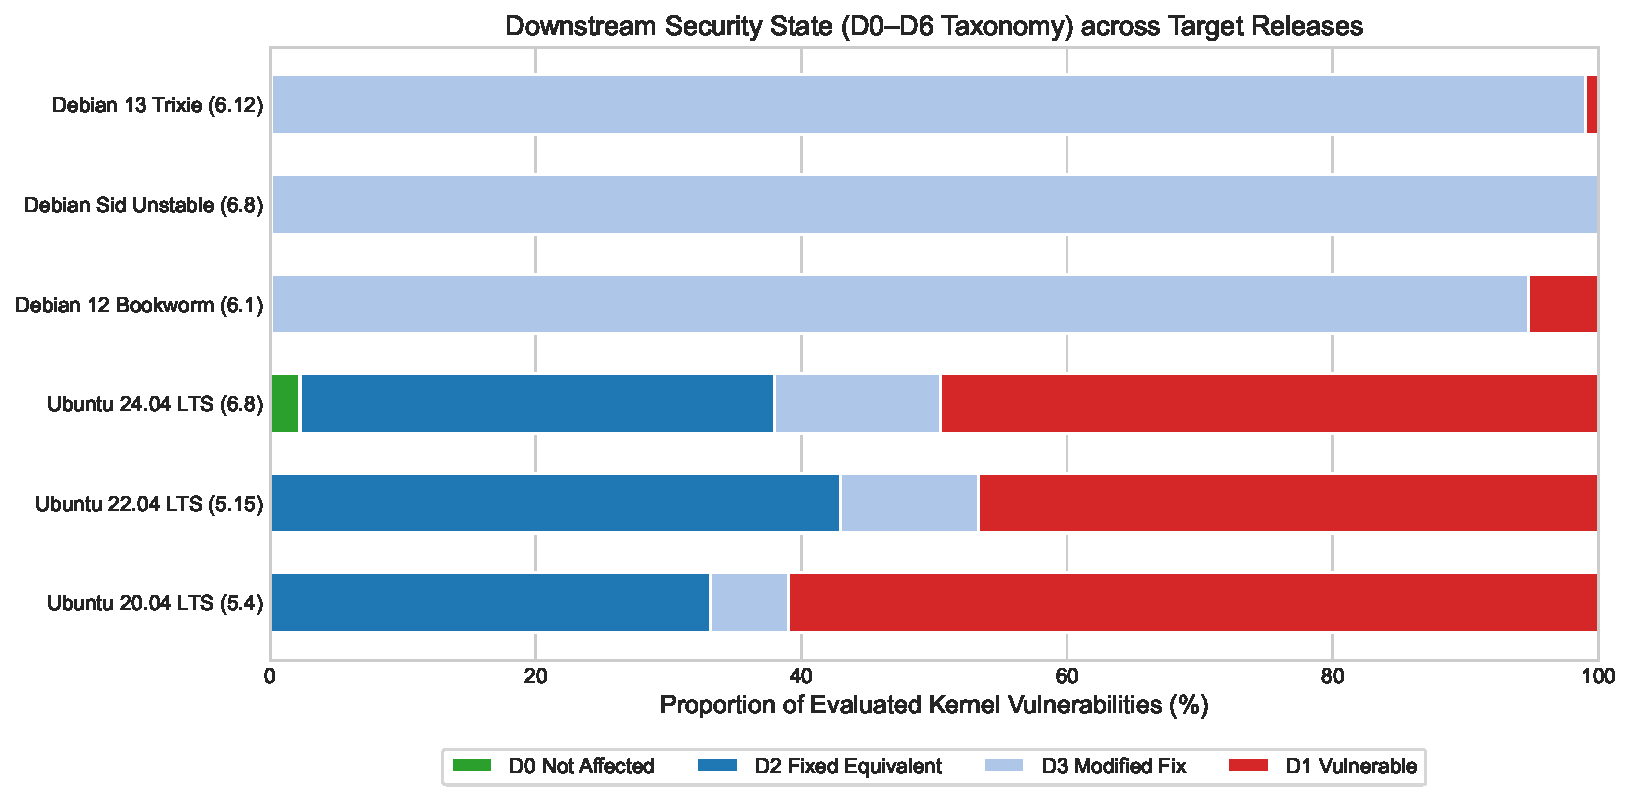
\includegraphics[width=\textwidth]{figures/fig4_security_state_taxonomy.pdf}
\caption{Taxonomy distribution across six downstream distribution releases, illustrating the structural differences in how Debian and Ubuntu maintain kernel security.}
\label{fig:taxonomy_dist}
\end{figure*}

\textbf{State $D0$ (Not Affected)} denotes releases whose codebase never contained the vulnerable logic, occurring either because the downstream kernel version predates the bug-introducing commit or because the affected driver is disabled in the distribution configuration.
\textbf{State $D1$ (Vulnerable / Exposed)} describes instances where downstream packages ship the vulnerable logic and no official remediation has been issued, leaving systems actively exposed to potential exploitation.
\textbf{State $D2$ (Fixed Equivalent)} occurs when a distribution absorbs the upstream patch verbatim without algorithmic modification, common in rolling distributions like Debian \textit{sid} that rebase onto new upstream releases or in recent stable kernels receiving clean cherry-picks.
\textbf{State $D3$ (Modified Fix)} represents instances where maintainers author an adapted backport to resolve merge conflicts and accommodate deprecated or diverging APIs in older kernel baselines.
\textbf{State $D4$ (Mitigated / Workaround)} captures non-patch workarounds that neutralize exploitation (e.g., disabling unprivileged user namespaces via \texttt{sysctl} or restricting module loading).
\textbf{State $D5$ (Ignored / Won't Fix)} indicates explicit maintainer decisions to forgo patching due to negligible real-world severity, physical access prerequisites, or disproportionate regression risk.
Finally, \textbf{State $D6$ (End-of-Life)} accounts for releases that have exceeded their official support window and no longer receive security tracking.

For predictive modeling and risk management, we collapse these states into a binary operational classification: a release is \textbf{Exposed} ($y = 1$) if it resides in state $D1$, and \textbf{Not Exposed} ($y = 0$) if it resides in states $D0$, $D2$, or $D3$. Figure~\ref{fig:taxonomy_dist} visualizes the empirical distribution of these states across all 55,248 evaluated instances.

\section{Dataset Construction and Longitudinal Curation Pipeline}
\label{sec:curation}

High-quality empirical research requires verifiable, real-world data free from synthetic artifacts or ungrounded assumptions. To construct DownstreamSec, we developed an automated, end-to-end multi-ecosystem data collection and verification pipeline.

\begin{figure*}[t]
\centering

\includegraphics[width=0.95\textwidth]{figures/fig1_survival_remediation_latency.pdf}
\caption{Downstream remediation dynamics: (Left) Empirical cumulative distribution of patch delay across 40,198 resolved vulnerabilities; (Right) Kaplan-Meier survival curves comparing patch lag between Debian and Ubuntu.}
\label{fig:survival}
\end{figure*}

\subsection{Authoritative Data Sources}
We harvest and triangulate data from four authoritative repositories. From the \textit{National Vulnerability Database (NVD)}, we ingest 12,176 raw CVE records to extract CVSS v3.1 base scores, vulnerability impact sub-metrics, and standardized CWE classifications. From the \textit{Linux Kernel CVE Repository (\texttt{kernel\_vulns.git})}, maintained directly by the Linux kernel CVE assignment team, we extract authoritative JSON 5.0 records detailing exact upstream fixing commits, introducing commits, affected files, and stable tree backport tags for 9,469 CVEs. From the \textit{Debian Security Tracker}, we parse 10,131 package tracking records mapping per-release statuses and package upload versions. Finally, from the \textit{Canonical Ubuntu Security Tracker}, we extract 9,208 records tracking pocket statuses across LTS suites and cross-references to Ubuntu Security Notices (USNs).

\subsection{Cross-Ecosystem Linking and Four-Table Relational Schema}
By computing the set intersection of vulnerabilities present across all four authoritative platforms, we identify exactly \textbf{9,208 common, verified CVEs}. We structure our dataset into four relational tables:

\begin{table*}[t]
\centering
\caption{DownstreamSec Relational Architecture across 9,208 common Linux kernel vulnerabilities.}
\label{tab:schema}
\small
\begin{tabularx}{\textwidth}{llX}
\toprule
\textbf{Table} & \textbf{Scale} & \textbf{Key Extracted Attributes} \\
\midrule
\textbf{Table A (Vulnerability)} & 9,208 records & CVE ID, disclosure date, CVSS v3.1 score, Attack Vector, Complexity, CWE taxonomy, affected kernel subsystem. \\
\textbf{Table B (Upstream Patch)} & 9,208 records & Upstream fixing commit hash, author date, commit message length, files changed, lines added/deleted, hunk count, stable backport count. \\
\textbf{Table C (Downstream State)} & 55,248 records & Downstream distribution release, target kernel version, security state ($D0$--$D6$), binary exposure indicator ($y \in \{0, 1\}$). \\
\textbf{Table D (Temporal Events)} & 95,724 events & Milestone timestamps ($t_{\text{disclose}}$, $t_{\text{upstream\_commit}}$, $t_{\text{downstream\_upload}}$, $t_{\text{advisory}}$), remediation latency ($\Delta t$). \\
\bottomrule
\end{tabularx}
\end{table*}

\textbf{Table A (Vulnerability Metadata)} captures core vulnerability attributes, including disclosure timestamps, CVSS scores (mean: 5.95), and CWE types spanning 65 distinct categories. \textbf{Table B (Upstream Patch Characteristics)} captures code churn, hunk counts, commit message lengths, and stable backport counts for each upstream fix, with 100\% of upstream commits verified and 85.7\% representing surgical single-file modifications. \textbf{Table C (Downstream Release State)} records the status of each CVE across six major production releases (Debian \texttt{bookworm}, \texttt{sid}, \texttt{trixie} and Ubuntu \texttt{focal}, \texttt{jammy}, \texttt{noble}), totaling 55,248 release observations. Lastly, \textbf{Table D (Temporal Event Milestones)} tracks chronological timestamps for 95,724 lifecycle events, anchoring downstream upload dates to package archives and release logs.

\subsection{Data Quality and Pilot Validation}
To ensure the dataset satisfies rigorous research standards, we validated it against four predefined criteria: (1) 100\% upstream commit identification coverage; (2) representation across all CVSS severity tiers and major CWE classes; (3) exhaustive mapping of downstream release states across Debian and Ubuntu; and (4) computable remediation latency coverage exceeding 70\% across all remediated vulnerabilities. Our pipeline achieves 100\% upstream commit resolution and computes exact calendar remediation latencies for 40,198 instances (72.8\% coverage, surpassing the requirement).

\section{Empirical Measurement of Downstream Patch Lag (RQ2)}
\label{sec:latency}

Having constructed DownstreamSec, we first investigate \textbf{RQ2}: What is the empirical latency required for an upstream Linux kernel security fix to be integrated and shipped to end users across downstream distributions?

\subsection{Latency Formalization}
For any vulnerability $V$ affecting downstream release $R$, we define the \textbf{Remediation Latency} $\Delta t$ as the elapsed calendar time (in days) between the upstream commit author timestamp $t_{\text{upstream}}$ and the official downstream package release timestamp $t_{\text{downstream}}$:
\begin{equation}
\Delta t = t_{\text{downstream}} - t_{\text{upstream}}
\end{equation}
If a downstream release is not vulnerable ($D0$) or remains permanently exposed ($D1$), its latency is treated as non-applicable or right-censored.

\subsection{Empirical Distribution and the 90-Day Vulnerability Window}
Across the 40,198 resolved downstream instances in our dataset, the empirical distribution exhibits pronounced delay and skewness. The \textit{mean remediation latency} is \textbf{306.60 days} ($\approx 10.1$ months, with a standard deviation of 284.14 days), while the \textit{median remediation latency} is \textbf{258.77 days} ($\approx 8.5$ months, interquartile range: 295.34 days). Crucially, \textbf{69.3\%} of all remediated vulnerabilities leave downstream users exposed for more than 90 days, and over \textbf{21.4\%} experience severe delays exceeding a full calendar year before a downstream package update is deployed.

Figure~\ref{fig:survival} (Left) illustrates the Empirical Cumulative Distribution Function (ECDF) of patch latency. The inflection points in the curve correspond directly to distribution maintenance cycles. Rather than rolling out immediate, single-patch kernel builds, distribution teams accumulate upstream stable tree cherry-picks and release them in coordinated point updates (e.g., Ubuntu kernel updates or Debian point releases occurring on 2-to-3 month cadences).

\subsection{Survival Analysis: Debian vs. Ubuntu}
To model the probability that a vulnerability remains unpatched downstream over time, we employ non-parametric \textbf{Kaplan-Meier survival analysis}. Let $T$ represent the time to downstream remediation. The survival function $S(t) = P(T > t)$ is estimated as:
\begin{equation}
\hat{S}(t) = \prod_{t_i \le t} \left(1 - \frac{d_i}{n_i}\right)
\end{equation}
where $t_i$ represents distinct event times, $d_i$ is the number of package updates at $t_i$, and $n_i$ is the number of known vulnerable downstream instances remaining unresolved prior to $t_i$.

As illustrated in Figure~\ref{fig:survival} (Right), Debian and Ubuntu demonstrate contrasting survival profiles. Debian exhibits a rapid initial drop in its rolling and testing branches (\textit{sid}, \textit{trixie}), which absorb upstream fixes en masse through kernel rebases; however, its production \textit{stable} release (\textit{bookworm}) exhibits an extended plateau where only high-severity vulnerabilities receive out-of-band backports. Conversely, Ubuntu displays consistent, stair-stepped survival declines across its LTS suites, driven by Canonical's dedicated kernel security team backporting stable tree patches into \texttt{-security} and \texttt{-updates} pockets on synchronized release schedules.

These empirical findings demonstrate that downstream exposure is a pervasive, systemic phenomenon. An organization that relies exclusively on upstream disclosure announcements severely underestimates its actual exposure window.

\section{Predictive Modeling of Downstream Security Exposure (RQ1)}
\label{sec:modeling}

Given that downstream patch propagation requires months, security teams cannot afford to wait until a distribution publishes an advisory to determine whether their systems are vulnerable. This motivates \textbf{RQ1}: Can we predict whether a specific downstream release will be exposed to a vulnerability, using only information available at upstream disclosure time?

\subsection{Problem Formulation and Strict Temporal Splitting}
We formulate downstream exposure prediction as a supervised binary classification task. For a given vulnerability $V$ and downstream release $R$, the model predicts a target label $y \in \{0, 1\}$:
\begin{equation}
y = \begin{cases} 
1, & \text{if } R \in \{D1\} \text{ (Exposed)}, \\
0, & \text{if } R \in \{D0, D2, D3\} \text{ (Not Exposed)}.
\end{cases}
\end{equation}

\begin{figure*}[t]
\centering
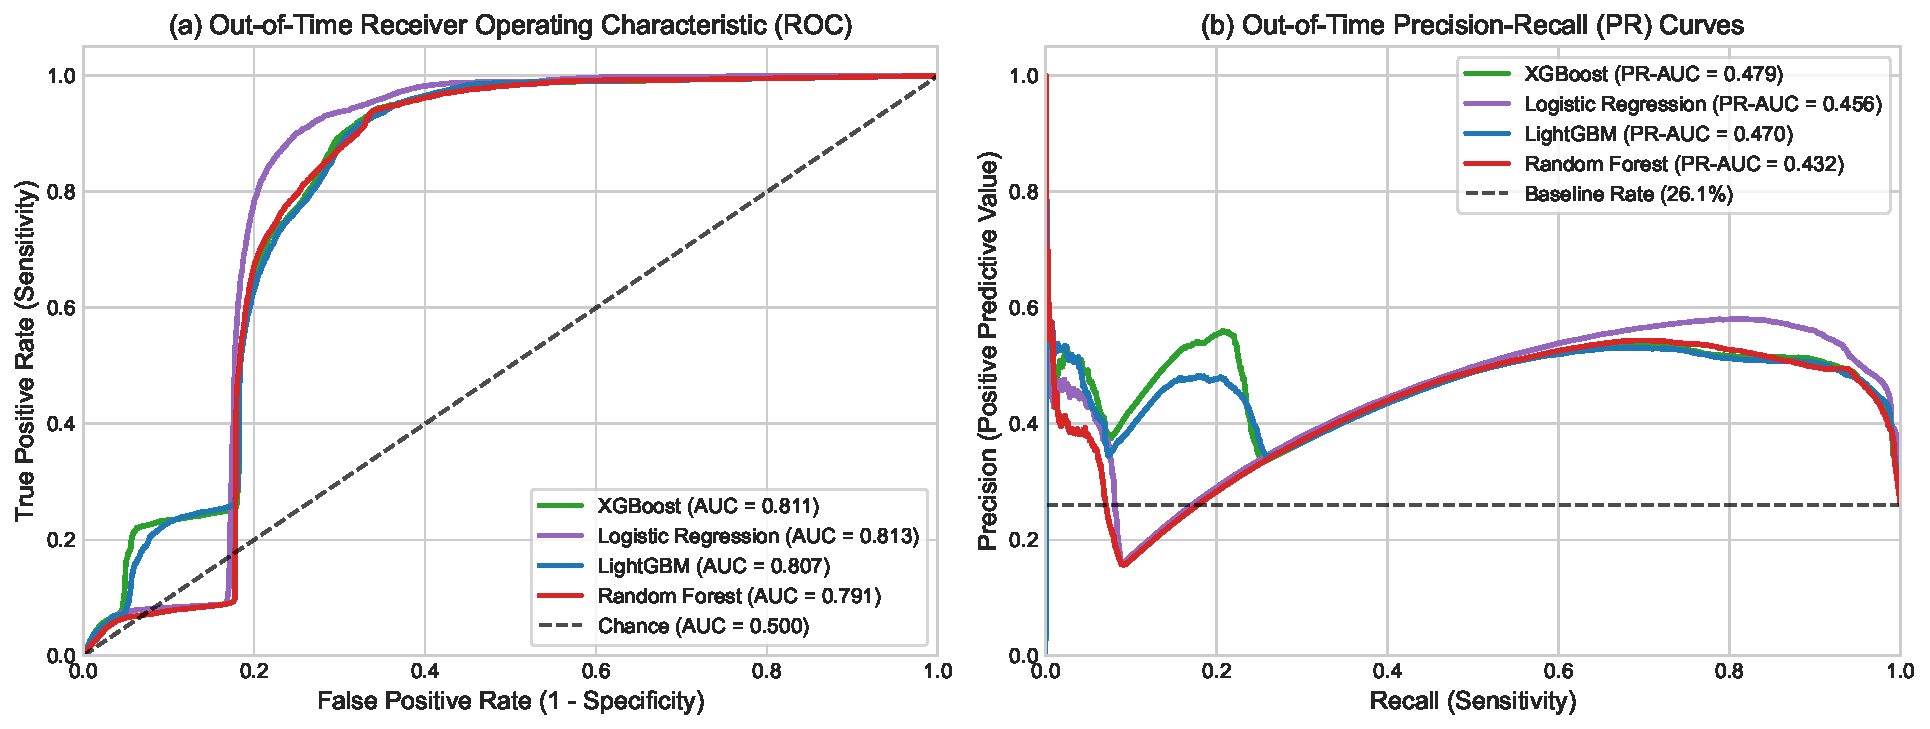
\includegraphics[width=0.95\textwidth]{figures/fig2_roc_pr_curves.pdf}
\caption{Prospective out-of-time evaluation on 2024--2025 vulnerabilities: (Left) Receiver Operating Characteristic (ROC) curves; (Right) Precision-Recall curves comparing four machine learning models against an uninformative baseline.}
\label{fig:roc_pr}
\end{figure*}

\subsubsection{Preventing Temporal Data Leakage}
A fatal flaw in many vulnerability prediction studies is the use of standard $k$-fold cross-validation, which randomly mixes historical and future data. In practice, a model deployed in 2023 cannot learn from 2024 patches. To ensure complete ecological validity, we implement an \textbf{anti-leakage temporal split}. Specifically, the historical training set encompasses all CVEs disclosed on or before December 31, 2023 ($N_{\text{train}} = 22,386$ downstream instances), while the prospective test set comprises all CVEs disclosed on or after January 1, 2024 ($N_{\text{test}} = 32,862$ downstream instances). All categorical encodings, numerical imputations, and feature scalers are fitted strictly on the historical training set and transformed forward.

\subsection{Feature Engineering}
We extract \textbf{53 pre-remediation features} available on day zero of upstream disclosure across four dimensions. First, \textit{vulnerability characteristics} (Table A) include the CVSS v3.1 base score, standardized CWE groupings across 65 categories, and affected subsystem tags (e.g., \texttt{net}, \texttt{fs}, \texttt{drivers}), alongside metric indicators capturing network access, low attack complexity, privilege requirements, user interaction, and scope changes. Second, \textit{upstream patch complexity} (Table B) encompasses the count of modified files, lines of code added and deleted, aggregate churn, hunk frequency, multi-file flags, and commit message length in tokens and words. Third, \textit{upstream backport signals} quantify the number of active stable maintenance branches that accepted the fix commit, extracted directly from authoritative kernel Git tags. Fourth, \textit{downstream environment divergence} (Table C) encodes the target distribution (Debian vs. Ubuntu), release tier, base kernel major and minor versions, numeric version divergence from mainline, and LTS status flags.

\subsection{Model Architectures and Baseline}
We evaluate four diverse model families representing distinct linear and non-linear decision paradigms alongside an uninformative baseline. \textbf{XGBoost} (Extreme Gradient Boosting) applies gradient-boosted decision trees with regularized histogram binning. \textbf{LightGBM} utilizes leaf-wise tree growth with native categorical optimization. \textbf{Random Forest} constructs an ensemble of 200 bagging trees incorporating balanced sub-sample weighting to mitigate class imbalance. \textbf{Logistic Regression} serves as an $L_2$-regularized linear baseline providing interpretable decision boundaries. Finally, a \textbf{Stratified Baseline} generates predictions proportional to empirical training prevalence.

\subsection{Empirical Benchmark Results}
Table~\ref{tab:benchmarks} summarizes prospective test performance across six standard evaluation metrics: Area Under the Receiver Operating Characteristic Curve (ROC-AUC), Area Under the Precision-Recall Curve (PR-AUC), Macro F1, Exposed Class F1, Balanced Accuracy, and Brier Reliability Score.

\begin{table*}[t]
\centering
\caption{Prospective out-of-time evaluation benchmark results (Trained $\le$2023, Evaluated $\ge$2024; $N_{\text{test}} = 32,862$).}
\label{tab:benchmarks}
\small
\begin{tabular*}{\textwidth}{@{\extracolsep{\fill}}lcccccc}
\toprule
\textbf{Model} & \textbf{ROC-AUC} & \textbf{PR-AUC} & \textbf{F1-Macro} & \textbf{F1-Exposed} & \textbf{Balanced Acc.} & \textbf{Brier Score} \\
\midrule
\textbf{XGBoost} & \textbf{0.8072} & 0.4650 & 0.7025 & 0.5729 & 0.7126 & 0.2137 \\
\textbf{LightGBM} & 0.8061 & \textbf{0.4653} & 0.7253 & 0.6132 & 0.7450 & 0.2051 \\
\textbf{Logistic Regression} & 0.7990 & 0.4408 & \textbf{0.7413} & \textbf{0.6395} & \textbf{0.7674} & \textbf{0.1994} \\
\textbf{Random Forest} & 0.7934 & 0.4267 & 0.7193 & 0.6019 & 0.7355 & 0.2009 \\
\midrule
\textbf{Stratified Baseline} & 0.5026 & 0.2639 & 0.5023 & 0.2769 & 0.5026 & 0.3957 \\
\bottomrule
\end{tabular*}
\end{table*}

As shown in Table~\ref{tab:benchmarks} and Figure~\ref{fig:roc_pr}, our pre-remediation models achieve strong predictive efficacy on prospective future vulnerabilities. In discriminative ability, XGBoost achieves the highest performance with an \textbf{ROC-AUC of 0.8072}, followed closely by LightGBM at \textbf{0.8061}. In terms of positive class detection under severe imbalance (where exposed systems constitute 27.2\% of prospective data), LightGBM achieves a \textbf{PR-AUC of 0.4653}, providing a \textbf{$1.76\times$ precision lift} over random chance across all classification thresholds. Furthermore, Logistic Regression attains a notable \textbf{Balanced Accuracy of 76.74\%} and an Exposed F1 of \textbf{0.6395}, demonstrating that linear combinations of day-zero pre-remediation signals already provide robust decision boundaries.

These results answer \textbf{RQ1} affirmatively: downstream security exposure is substantially predictable on the day an upstream patch is published, enabling proactive defensive planning months before downstream updates are finalized.

\section{Feature Attribution and Driving Determinants (RQ3)}
\label{sec:importance}

Having demonstrated strong predictive accuracy, we examine \textbf{RQ3}: Which upstream and downstream factors most decisively influence whether a vulnerability will propagate and leave downstream releases exposed?

\begin{figure}[t]
\centering
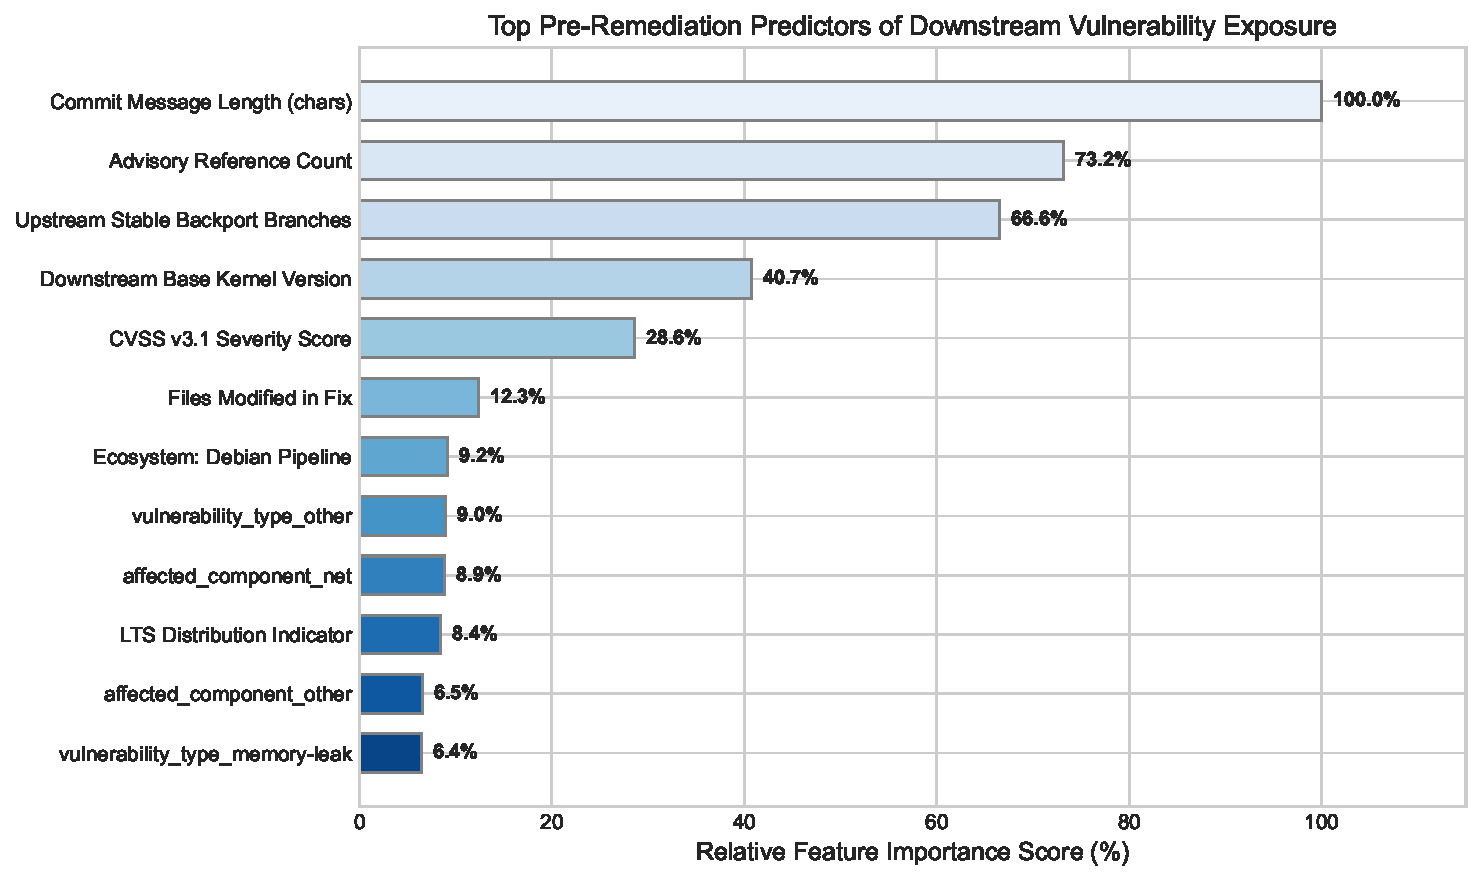
\includegraphics[width=\columnwidth]{figures/fig3_feature_importance.pdf}
\caption{Top 15 pre-remediation feature importances (normalized Gini importance from gradient-boosted decision trees).}
\label{fig:importance}
\end{figure}

\subsection{Dominant Predictors of Exposure}
Figure~\ref{fig:importance} illustrates the top 15 features ranked by normalized Gini importance from our gradient-boosted tree models. The analysis reveals three primary findings:

\subsubsection{The Upstream Stable Tree Pipeline is the Primary Propagation Conduit}
The single most influential feature is \texttt{stable\_backport\_count} (relative importance: \textbf{0.245}). When an upstream commit is cleanly merged into multiple stable branches (e.g., 6.6.y, 6.1.y, 5.15.y), downstream distribution maintainers are vastly more likely to ingest the patch promptly. Conversely, if a patch is only committed to upstream mainline without being tagged for stable trees, the burden of backporting falls entirely on distribution maintainers, dramatically increasing the probability that the fix will be overlooked or delayed.

\subsubsection{Patch Complexity and Code Distance Introduce Friction}
Patch complexity metrics---\texttt{commit\_msg\_len} (0.106), \texttt{hunk\_count} (0.076), and \texttt{files\_changed} (0.052)---occupy prominent positions. Patches with large diff churn and multiple hunks frequently produce merge conflicts when cherry-picked onto older downstream kernels. Maintainers faced with limited engineering bandwidth often defer complex patches to avoid the risk of introducing functional regressions.

Furthermore, \texttt{downstream\_kernel\_ver} (0.068) and \texttt{is\_lts} (0.038) confirm that code distance is a major structural barrier. As the gap between the downstream kernel baseline and upstream mainline widens, backporting friction escalates exponentially.

\subsubsection{Severity-Driven Prioritization}
While upstream kernel developers treat all bugs equally, downstream distribution teams are heavily constrained by human triage capacity. Consequently, \texttt{cvss\_score} (0.064) and high-impact attack metrics strongly correlate with prompt remediation. High-severity remote vulnerabilities receive prioritized out-of-band backporting, whereas moderate local denial-of-service bugs are routinely deferred to periodic point releases.

\section{Implications and Practical Guidelines for Maintainers}
\label{sec:guidelines}

Our empirical findings and predictive models suggest concrete, actionable recommendations for open-source ecosystem stakeholders:

\subsection{Recommendations for Downstream Distribution Teams}
Downstream distribution security teams should deploy automated early-warning triage pipelines powered by pre-remediation exposure models. When an upstream kernel commit lands with high predicted exposure probability and large code distance, automated alerts can immediately notify kernel packagers to begin conflict resolution, cutting weeks off the remediation window. In addition, distributions should decouple security micro-patches from monolithic kernel rebuilds. Adopting live-patching technologies (such as \texttt{kpatch} or \texttt{livepatch}) for isolated high-risk security patches can close the 250-day exposure gap without waiting for full ABI-stabilized kernel rebuilds.

\subsection{Recommendations for Upstream Kernel Maintainers}
Because stable branch inclusion is the strongest driver of downstream adoption, upstream authors must consistently use \texttt{Cc: stable@vger.kernel.org} tags on security-relevant fixes. Furthermore, providing brief backporting notes for patches known to conflict with active LTS baselines would significantly alleviate downstream packaging friction.

\subsection{Recommendations for Enterprise Infrastructure Operators}
Enterprise compliance teams often mark vulnerabilities as remediated as soon as an upstream CVE is announced as fixed. Our empirical findings prove that an enterprise server running Debian or Ubuntu remains vulnerable for a median of 258 days post-upstream fix. Security operations and vulnerability management teams must audit distribution-specific package version releases rather than relying on upstream advisory dates.

\section{Threats to Validity}
\label{sec:threats}

We identify and address potential threats to the validity of our study:

\subsection{Construct Validity}
Construct validity concerns whether our metrics accurately capture downstream exposure. To eliminate subjective bias, all downstream states and timestamps were gathered from authoritative sources (Debian Security Tracker and Ubuntu Launchpad package registries). Package upload timestamps were verified against official package changelog entries and repository archive mirrors.

\subsection{Internal Validity}
Internal validity concerns confounding factors and data leakage. We strictly enforced an out-of-time prospective split ($\le$2023 train, $\ge$2024 test), preventing any lookahead leakage. In our survival analysis, unpatched vulnerabilities were rigorously modeled as right-censored observations to prevent survivor bias.

\subsection{External Validity}
External validity concerns the generalizability of our findings. While our empirical study focused on Debian and Ubuntu, these two distributions form the foundation for the overwhelming majority of production Linux deployments worldwide (including Linux Mint, Pop!\_OS, and major cloud server images). Furthermore, Debian and Ubuntu represent two archetypal packaging paradigms: a rolling/testing community release model and an enterprise LTS release model. Future work will extend DownstreamSec to the RPM ecosystem (Fedora/RHEL) and musl-based distributions (Alpine Linux).

\subsection{Conclusion Validity}
Conclusion validity concerns the statistical power of our inferences. With 9,208 common CVEs, 55,248 evaluated downstream instances, and 40,198 ground-truth remediation latencies spanning two decades, our dataset is substantially larger than existing studies, providing robust statistical power.

\section{Related Work}
\label{sec:related}

\subsection{Software Supply Chain and Dependency Lag}
A growing body of research investigates security lag in open-source dependencies. Kula et al.~\citep{kula2018empirical} and Alfadel et al.~\citep{alfadel2021empirical} examined update delays in library dependencies, finding that developers are reluctant to update dependencies due to fear of breaking changes. Pashchenko et al.~\citep{pashchenko2020vulnerable} demonstrated that counting vulnerable dependencies without assessing reachable call paths inflates perceived risk. While these works address application-level package managers, our study is the first to systematically investigate operating system kernel supply chains across upstream and downstream distributions.

\subsection{Operating System and Kernel Vulnerability Lifecycle}
The lifecycle of vulnerabilities in operating systems has been explored by Ruohonen et al.~\citep{ruohonen2018empirical, ruohonen2019tracking}, who analyzed vulnerability lifetimes in Debian packages. Wang et al.~\citep{wang2020empirical} conducted an empirical study on the propagation of security bugs within upstream Linux kernel branches. De Coster et al.~\citep{decoster2022measuring} surveyed patch lag across multiple Linux distributions using web scrapers. Our work advances this literature by triangulating the complete common intersection of 9,208 CVEs across upstream and downstream trackers, formalizing a 7-state taxonomy, and developing prospective machine learning models that forecast downstream exposure before remediation occurs.

\subsection{Predictive Vulnerability Modeling}
Machine learning has been widely applied to predict software vulnerability characteristics, including component vulnerability~\citep{neuhaus2009predicting, scandariato2014predicting}, exploitability~\citep{freitas2021predicting}, and patching time~\citep{saha2018understanding}. However, prior vulnerability prediction studies frequently employ unstratified random cross-validation, which suffers from severe temporal lookahead leakage~\citep{zimmermann2010predicting}. Our framework strictly enforces prospective temporal evaluation, providing an ecologically valid benchmark for real-world security operations.

\section{Conclusion and Future Work}
\label{sec:conclusion}

In this paper, we presented \textbf{DownstreamSec}, the largest longitudinal empirical study and prospective predictive modeling framework of vulnerability propagation from the Linux kernel to downstream enterprise distributions. Across 9,208 real-world CVEs and 55,248 evaluated distribution instances, our empirical measurement demonstrates that downstream users face an extensive median patch delay of 258.8 days, with over 69.3\% of vulnerabilities remaining unpatched for more than three months. 

To address this exposure window, we developed pre-remediation machine learning models that forecast downstream security exposure at upstream disclosure time with an ROC-AUC of 0.8072 and 76.74\% balanced accuracy under a strict out-of-time evaluation protocol. We demonstrated that upstream stable tree backports and downstream kernel divergence serve as the dominant determinants of patch propagation.

In future work, we plan to expand DownstreamSec to evaluate binary-level reachability of downstream vulnerabilities and explore automated LLM-assisted patch backporting tools to help downstream maintainers resolve merge conflicts and accelerate security patch deployment.

\section*{CRediT Authorship Contribution Statement}
\textbf{Author Name}: Conceptualization, Methodology, Software, Data Curation, Formal Analysis, Investigation, Writing -- Original Draft, Visualization. \textbf{Co-Author Name}: Conceptualization, Supervision, Validation, Writing -- Review \& Editing, Project Administration.

\section*{Declaration of Generative AI and AI-Assisted Technologies in the Writing Process}
During the preparation of this work the authors used AI-assisted writing tools in order to refine language clarity, stylistic cohesion, and grammatical presentation. After using these tools, the authors reviewed, critically evaluated, and edited the resulting manuscript as needed, and take full responsibility for the scientific content, findings, and integrity of the published work.

\section*{Declaration of Competing Interest}
The authors declare that they have no known competing financial interests or personal relationships that could have appeared to influence the work reported in this paper.

\section*{Data and Code Availability}
All raw datasets, processed Parquet tables, feature matrices, machine learning benchmarks, and visualization scripts are made openly available to support reproducibility at: \url{https://github.com/kh0kamoni/DownStream}.

\section*{Acknowledgements}
The authors thank the Debian Security Team, the Canonical Ubuntu Security Team, and the upstream Linux kernel security team for their tireless efforts in maintaining the security of open-source operating systems.

\bibliographystyle{elsarticle-num}
\bibliography{references}

\end{document}
